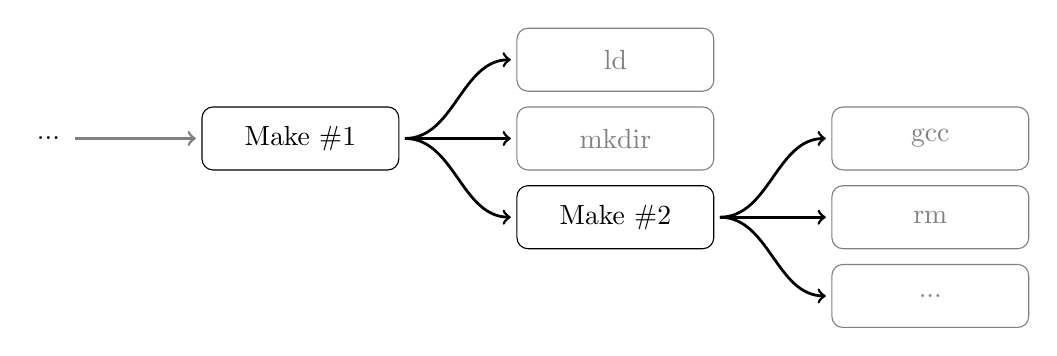
\begin{tikzpicture}
    \node (tracer) at (3.8, 0) {...};
    \node[minimum width=2.5cm, minimum height=0.8cm, style=draw, rounded corners] (make) at (7, 0) {Make~\#1};
    \node[minimum width=2.5cm, minimum height=0.8cm, gray, style=draw, rounded corners] (child1) at (11, 1) {ld};
    \node[minimum width=2.5cm, minimum height=0.8cm, gray, style=draw, rounded corners] (child2) at (11, 0) {mkdir};
    \node[minimum width=2.5cm, minimum height=0.8cm, style=draw, rounded corners] (child3) at (11, -1) {Make~\#2};

    \node[minimum width=2.5cm, minimum height=0.8cm, gray, style=draw, rounded corners] (child31) at (15, 0) {gcc};
    \node[minimum width=2.5cm, minimum height=0.8cm, gray, style=draw, rounded corners] (child32) at (15, -1) {rm};
    \node[minimum width=2.5cm, minimum height=0.8cm, gray, style=draw, rounded corners] (child33) at (15, -2) {...};

    \draw[gray, line width=1pt, shorten >=2pt, shorten <=2pt, ->] (tracer) -- (make);
    \draw[line width=1pt, shorten >=2pt, shorten <=2pt, ->] (make) to[in=180, out=0] (child1);
    \draw[line width=1pt, shorten >=2pt, shorten <=2pt, ->] (make) to[in=180, out=0] (child2);
    \draw[line width=1pt, shorten >=2pt, shorten <=2pt, ->] (make) to[in=180, out=0] (child3);

    \draw[line width=1pt, shorten >=2pt, shorten <=2pt, ->] (child3) to[in=180, out=0] (child31);
    \draw[line width=1pt, shorten >=2pt, shorten <=2pt, ->] (child3) to[in=180, out=0] (child32);
    \draw[line width=1pt, shorten >=2pt, shorten <=2pt, ->] (child3) to[in=180, out=0] (child33);

    % \node[gray, font=\small] (text1) at (6.7, -2) {События ptrace};
    % \node[gray, font=\small] (text1) at (1, -2) {События над файлами и процессами};
    % \node[gray, font=\small] (text2) at (3.5, 1.8) {Соответствие процессов целям и граф зависимостей};
\end{tikzpicture}